\documentclass{llncs}

\sloppy

\usepackage{lmodern}
\usepackage{amsmath}
\usepackage{amssymb}
\usepackage{amsfonts}
\usepackage{alltt}
\usepackage{paralist}
\usepackage{caption}
\usepackage{subcaption}
\usepackage{xspace}
\usepackage{mdwtab}
\usepackage{multirow}
\usepackage[square,numbers,sort&compress,comma,sectionbib]{natbib}
\usepackage{wrapfig}
\usepackage{algorithm}
\usepackage[noend]{algpseudocode}
\usepackage{tikz}
\usepackage{pgfplots}
\pgfplotsset{compat=1.12}
\usepackage{hyperref}

\newcommand\comment[1]{}
\newcommand\arsays[1]{{\bf AR: #1}}
\newcommand\ausays[1]{{\bf AU: #1}}

\newcommand{\ie}{\emph{i.e.}}
\renewcommand{\bibname}{References}
\newcommand\Integers{\mathbb{Z}}
\newcommand\tuple[1]{\langle #1 \rangle}
\newcommand\True{\mathit{True}}
\newcommand\None{\mathit{None}}
\newcommand\Equiv{\mathit{Eq}}
\newcommand\Points{\mathit{Pts}}
\newcommand\Point{\mathit{Pt}}
\newcommand\Verify{\mathit{Verify}}
\newcommand\CexInput{\mathit{CexPt}}
\newcommand\Predicates{\mathit{Preds}}
\newcommand\Expr{e}
\newcommand\Pred{p}
\newcommand\Terms{\mathit{Terms}}
\newcommand\Term{t}
\newcommand\Cover{\mathit{Cover}}
\newcommand\Powerset[1]{\mathbf{2}^{#1}}
\newcommand\Spec{\Phi}
\newcommand\Size{K}
\newcommand\Grammar{G}
\newcommand\sem[1]{[\![ #1 ]\!]}
\newcommand\SynthFun{f}
\newcommand\range{\mathit{range}}
\newcommand\FormalParameters{\mathit{Params}}
\newcommand\Productions{\mathit{Prodn}}
\newcommand\Prob[1]{\mathbb{P}(#1)}
\newcommand\NonTerminals{\mathcal{N}}
\newcommand\NonTerminal{N}
\newcommand\StartSymbol{S}
\newcommand\Symbols{\mathit{Symbols}}
\newcommand\Rules{\mathcal{R}}
\newcommand\Rule{R}
\newcommand\Theory{\mathcal{T}}
\newcommand\RewritesTo{\rightarrow}
\newcommand\ITE[3]{\mathtt{if}~#1~\mathtt{then}~#2~\mathtt{else}~#3}

\newcommand\DecisionTree{\mathit{DT}}
\newcommand\DTtoExpr[1]{\mathit{Expr}(#1)}
\newcommand\NodesInternal{V_I}
\newcommand\Nodes{V}
\newcommand\node{v}
\newcommand\NodesLeaf{V_L}
\newcommand\EdgesYes{E_Y}
\newcommand\EdgesNo{E_N}
\newcommand\Edges{E}
\newcommand\Attribute{\mathcal{A}}
\newcommand\Label{\mathcal{L}}
\newcommand{\sygus}{{\sffamily\fontsize{8.5}{10}\selectfont
    SyGuS}\xspace}
\newcommand{\dcsolve}{{\sffamily\fontsize{8.5}{10}\selectfont
    DCSolve}\xspace}
\renewcommand{\paragraph}[1]{\par\noindent\textbf{#1}.}
\newcommand{\itparagraph}[1]{\par\noindent\textit{#1}.}
\newcommand{\esolver}{\textsc{esolver}\xspace}

% Make floats and equations behave sensibly
\setlength{\intextsep}{1pt}
\setlength{\textfloatsep}{1pt}
\setlength{\floatsep}{1pt}
\abovedisplayskip=6pt plus 3pt minus 9pt
\abovedisplayshortskip=0pt plus 3pt
\belowdisplayskip=6pt plus 3pt minus 9pt
\belowdisplayshortskip=7pt plus 3pt minus 4pt
\setlength\abovecaptionskip{1pt}
\setlength\belowcaptionskip{1pt}

\begin{document}
\pagestyle{plain}
\title{Scaling Enumerative Program Synthesis via Divide and Conquer}
% \author{Rajeev Alur \and Arjun Radhakrishna \and Abhishek Udupa}
\author{}
% \institute{University of Pennsylvania}
\institute{}
\maketitle
\vspace*{-6ex}

\begin{abstract}
  Given a semantic constraint specified by a logical formula and
  syntactic constraint specified by a context-free grammar, the
  Syntax-Guided Synthesis (SyGuS) problem is to find an expression
  that satisfies both the syntactic and semantic constraints.
  An enumerative approach to solve this problem is to systematically
  generates all expressions from the syntactic space with some pruning,
  and has proved to be surprisingly competitive in the newly started
  competition of SyGuS solvers.  It performs well on small to medium sized
  benchmarks, produces succinct expressions, and has the ability to
  generalize from input-output examples.  However, its performance
  degrades drastically with the size of the smallest solution. To overcome
  this limitation, in this paper we propose an alternative approach to
  solve SyGuS instances.

  The key idea  is to employ a divide-and-conquer approach by
  separately enumerating (a) smaller expressions that are correct on
  subsets of inputs, and (b) predicates on inputs that distinguish these
  subsets.  These smaller expressions and predicates are then combined
  using decision trees to obtain an expression that is correct on all
  inputs.  We view the problem of combining expressions and predicates as
  a multi-label decision tree learning problem. We propose a novel
  technique of associating a probability distribution over the set of
  labels that a sample can be labeled with. This enables us to use
  standard information-gain based heuristics to learn a compact decision
  tree.

  We report a prototype implementation and evaluate it on the benchmarks
  from the SyGuS 2015 competition. Our tool is able to match the running
  times and the succinctness of solutions of both standard enumerative
  solver as well as the latest white-box solvers in most cases.  Further,
  our solver is able to solve a large number of instances from the ICFP
  class of benchmarks, which were previously unsolved by all existing
  solvers.
\end{abstract}

\arsays{Change main algo to check for distinctness on points}

\section{Introduction}
\label{sec:intro}

\section{Illustrative Examples}
\label{sec:example}

Consider a

\arsays{Make an example where all pieces are generated at a small size,
but the full expression takes much longer}


\section{Problem Statement and Background}
\label{sec:problem}

Let us fix the function to be synthesized $\SynthFun$ and its formal
parameters $\FormalParameters$.
We write $\range(\SynthFun)$ to denote the range of $\SynthFun$.
The term {\em point} denotes a valuation of $\FormalParameters$, i.e., a
point is an input to $\SynthFun$.

\begin{example}
  For the running example in this section, we consider a function to be
  synthesized $\SynthFun$ of type $\Integers \times \Integers \to
  \Integers$ with the formal parameters $\FormalParameters = \{ x, y \}$.
  Points are valuations of $x$ and $y$.
  For example, $\{ x \mapsto 1, y \mapsto 2 \}$ is a point.
\end{example}

\paragraph{Specifications}
Satisfiability modulo theory formulae have become the standard formalism
for specifying semantic constraints for synthesis.
In the rest of this paper, we fix an arbitrary theory $\Theory$ and
denote by $\Theory[\Symbols]$, the set of $\Theory$ terms over the
symbols $\Symbols$.
A {\em specification} $\Spec$ is a logical formula in a theory $\Theory$
over standard theory symbols and the function to be synthesized
$\SynthFun$.
We say that an expression $\Expr$ satisfies a specification $\Spec$ if
instantiating the function to be synthesized $\SynthFun$ by $\Expr$
makes the formula $\Spec$ valid.

\begin{example}
  \label{ex:running:spec}
  Continuing the running example, we define a specification $\Spec
  \equiv \forall x, y : \SynthFun(x, y) \geq x \wedge \SynthFun(x, y)
  \geq y \wedge f(x, y) = x \vee f(x, y) = y$.
  The specification states that the function to be synthesized
  $\SynthFun$ maps each pair $x$ and $y$ to a value that is at least as
  great as each of them and equal to one of them.
  The function that returns the maximum of the two input values is the
  only possible function that satisfies this specification.
\end{example}

\paragraph{Grammars}
An {\em expression grammar} $\Grammar$ is a tuple $\tuple {
\NonTerminals, \StartSymbol, \Rules }$ where:
\begin{inparaenum}[(a)]
\item the set $\NonTerminals$ is a set of non-terminal symbols,
\item the non-terminal $\StartSymbol \in \NonTerminals$ is the initial non-terminal,
\item $\Rules \subseteq \NonTerminals \times
  \Theory[\NonTerminals \cup \FormalParameters]$ is a finite set
  of rewrite rules that map $\NonTerminals$ to $\Theory$-expressions
  over non-terminals and formal parameters.
\end{inparaenum}
We say that an expression $\Expr$ {\em rewrites to} an incomplete
expression $\Expr'$ (written as $\Expr \RewritesTo_\Grammar \Expr'$) if
there exists a rule $\Rule = (\NonTerminal, \Expr'') \in \Rules$ and
$\Expr'$ is obtained by replacing one occurrence of $\NonTerminal$ in
$\Expr$ by $\Expr''$.
Let $\RewritesTo_\Grammar^*$ be the transitive closure of $\RewritesTo$.
We say that an expression $\Expr \in \Theory[\FormalParameters]$
is {\em generated} by the grammar $\Grammar$ (written as $\Expr \in
\sem{\Grammar}$) if $\StartSymbol \RewritesTo_\Grammar^* \Expr$.
Note that we implicitly assume that all terms generated by the grammar
have the right type, i.e., are of the type $\range(\SynthFun)$.

\begin{example}
  \label{ex:running:grammar}
  For the running example, we choose the following grammar.
  The non-terminals are given by $\NonTerminals = \{ \StartSymbol, T, C \}$ with
  the initial non-terminal bein $\StartSymbol$.
  The rules are $\{ (\StartSymbol, T), (\StartSymbol,
        \mathtt{if}~C~\mathtt{then}~\StartSymbol~\mathtt{else}~\StartSymbol)
        \} \cup \{ (T, x), (T, y), (T, 1), (T, - T), (T, T + T) \} \cup
        \{ (C, T \leq T), (C, C \wedge C), (C, \neg C) \}$.
  This is the standard linear integer arithmetic grammar used for many
  SyGuS problems.
  Written in standard BCNF notation, this grammar is equivalent to:
    \vspace{-1ex}
  \begin{alltt}
    S ::= T | if (C) then T else T
    T ::= x | y | 1 | T + T | - T
    C ::= T \(\leq\) T | T < T | C \(\wedge\) C | \(\neg\) C
  \end{alltt}
    \vspace{-4ex}
\end{example}

\paragraph{The Syntax-Guided Synthesis Problem}
An instance of the SyGuS problem is given by a pair $\tuple { \Spec,
\Grammar }$ of specification and grammar.
An expression $\Expr$ is a solution to the instance if $\Expr \models
\Spec$ and $\Expr \in \sem{\Grammar}$.

\begin{example}
  Continuing the running example, for the specification $\Spec$ from
  Example~\ref{ex:running:spec} and the grammar from
  Example~\ref{ex:running:grammar}, one of the solution expressions is
  given by $\SynthFun(x, y) \equiv \mathtt{if}~x > y~\mathtt{then}~x~\mathtt{else}~y$.
\end{example}

From our definitions, it is clear that we restrict ourselves to a
version of the SyGuS problem where there is exactly one unknown function
to be synthesized, and the grammar does not contain {\tt let} rules.
Further, we assume that our specifications are {\em
  point-wise}\footnote{For brief discussion on different syntactic and
semantic notions of point-wise specifications, see the appendix}.
Intuitively, if a specification is point-wise, if it just relates the
input point to its output, and not the outputs of different inputs.

Here, we use a simple syntactic notion of point-wise specifications for
convenience.
However, our techniques can be generalized to any notion of point-wise
specifications.
Formally, we say that a specification is {\em plainly separable} if can
be rewritten into a conjunctive normal form where each clause is either
\begin{inparaenum}[(a)]
\item a tautology, or
\item every appearing application of the function to be synthesized
  $\SynthFun$ have the same arguments.
\end{inparaenum}

\begin{example}
  The specification for our running example $\Spec \equiv \SynthFun(x,
  y) \geq x \wedge \SynthFun(x, y) \geq y \wedge \SynthFun(x, y) = x
  \vee \SynthFun(x, y) = y$ is plainly separable.
  For example, this implies that the value of $\SynthFun(1, 2)$ can be
  chosen irrespective of the value of $\SynthFun$ on any other point.
  On the other hand, a specification such as $\SynthFun(x, y) = 1
  \implies \SynthFun(x + 1, y) = 1$ is neither plainly separable nor
  point-wise.
  The value of $\SynthFun(1, 2)$ cannot be chosen independently of the
  value of $\SynthFun(0, 2)$.
\end{example}

Point-wise (and in turn, simply separable) specifications allow us to
define the notion of an expression $\Expr$ satisfying a specification
$\Spec$ on a point $\Point$.
\arsays{Formally, we say that $\Expr \models \Spec \downharpoonleft
\Point$ if \dots}
We extend this definition to sets of points as follows: $\Expr \models
\Spec \downharpoonleft \Points \Leftrightarrow \bigwedge_{\Point \in
\Points} \Expr \models \Spec\downharpoonleft\Point$.

\begin{example}
  \label{ex:running:correctness_on_point}
  For the specification $\Spec$ of the running example, the function
  given by $\SynthFun(x, y) \equiv x + y$ is correct on the point $\{ x
      \mapsto 0, y \mapsto 3 \}$ and incorrect on the point $\{ x
  \mapsto 1, y \mapsto 2 \}$
\end{example}

The above restrictions make the SyGuS problem significantly easier.
However, a large number of problems do fall into this class (\arsays{x
out of y benchmarks in the SyGuS 2015 competition}).
Several previous works address this class of problem (see, for
example, \cite{ACR15,Madhu,xxx}).
The following example shows that a number of commonly occurring
specification mores are point-wise specifications.

\subsection{The Enumerative Solver}
\label{sec:enumeration}

\begin{wrapfigure}{l}{0.5\textwidth}
  \begin{minipage}{0.5\textwidth}
    \begin{algorithm}[H]
      \begin{algorithmic}[1]
        \Require Grammar $\Grammar = \tuple { \NonTerminals, \StartSymbol, \Rules }$
        \Require Specification $\Spec$
        \Ensure $\Expr$ s.t.  $\Expr \in \sem{\Grammar} \wedge \Expr \models \Spec$
        \State $\Point \gets \emptyset$ \label{line:basic:init}
        \While { $\True$ }
        \For {$\Expr \in \Call{Enumerate}{\Grammar,\Points}$ }\label{line:basic:enumerate}
        \If { $\Expr \models \Spec \downharpoonleft  \Points$ } \textbf{continue} \EndIf\label{line:basic:concrete_check}
        \State $\CexInput \gets \Verify(\Expr, \Spec)$ \label{line:basic:verify}
        \If { $\CexInput = \bot$ } \Return $\Expr$ \EndIf \label{line:basic:return}
        \State $\Points \gets \Points \cup \CexInput$ \label{line:basic:continue}
        \EndFor
        \EndWhile
      \end{algorithmic}
      \caption{Enumerative Solver}
      \label{algo:basic}
    \end{algorithm}
  \end{minipage}
\end{wrapfigure}
The principal idea behind the enumerative solver is to enumerate all
expressions from the given syntax with some pruning.
Only expressions that are distinct with respect to a set of concrete
input points are enumerated.

The full pseudo-code is given in Algorithm~\ref{algo:basic}.
Initially, the set of points is empty (line~\ref{line:basic:init}).
In each iteration, the algorithm calls the {\tt Enumerate} procedure
which returns a (possibly infinite) list of expressions that are all
distinct with respect to $\Points$ (line~\ref{line:basic:enumerate}).
This $\Expr$ is then verified, first on the set of points
(line~\ref{line:basic:concrete_check}) and then fully
(line~\ref{line:basic:verify}).
If the expression $\Expr$ is correct, it is returned
(line~\ref{line:basic:return}).
Otherwise, we pick a counter-example input point (i.e., an input on
which $\Expr$ is incorrect) and add it to the set of points and repeat
(line~\ref{line:basic:continue}).

For completeness, we recall the {\tt Enumerate} procedure here
(Algorithm~\ref{algo:enumerate}).
\footnote{Note that {\tt Enumerate} is a coprocedure.
  Unfamiliar readers may assume that each call to {\tt
  Enumerate} returns the next expression from an infinite list of
expressions}
It maintains a map $\Productions : \NonTerminals \to
\Powerset{\Theory[\FormalParameters]}$ from non-terminals to
expressions they can produce.
The invariant maintained by the procedure is that every pair of
expressions in $\Productions[\NonTerminal]$ is distinct on $\Points$.

The algorithm starts by first accumulating into
$\Productions[\NonTerminal]$ the expressions that can be produced from
$\NonTerminal$ in one step
(lines~\ref{line:enumerate:level_one_iter}-\ref{line:enumerate:level_one}).
Then, for each possible expression size $\Size$, it attempts to
instantiate each production rule in the grammar with expressions already
generated and stored in $\Productions$, to generate new expressions of
size at most $\Size$.
These newly generated expression are checked for distinctness from
already generated ones, and if so, added to
$\Productions[\NonTerminal]$.
The algorithm returns all the expressions produced from the starting
non-terminal $\StartSymbol$.

\begin{algorithm}
  \begin{algorithmic}[1]
    \Require Grammar $\Grammar = \tuple { \NonTerminals, \StartSymbol, \Rules }$ and a set of points $\Points$
    \Ensure Expressions $\tuple { \Expr_1, \Expr_2, \ldots }$ s.t. $\forall i < j : \vert \Expr_i \vert \leq \vert \Expr_j
    \vert \wedge \exists \Point \in \Points : \Expr_i[\Point] \neq \Expr_j[\Point]$
    \ForAll {$\NonTerminal \in \NonTerminals$} $\Productions[\NonTerminals] \gets \emptyset$ \EndFor
    \ForAll {$(\NonTerminal, \Expr) \in \Rules$}\label{line:enumerate:level_one_iter}
    \If { $\Expr \in \Theory[\FormalParameters]$ }
    $\Productions[\NonTerminal] \gets \Productions[\NonTerminal] \cup \{ \Expr \}$  \label{line:enumerate:level_one}
    \EndIf
    \EndFor
    \State $ \Size \gets 1 $
    \While { $\True$ }
    \ForAll {$(\NonTerminal, \Expr) \in \Rules$}
    \State $(\NonTerminal_1, \ldots, \NonTerminal_n) \gets \mbox{List of non-terminals occurring in $\Expr$ }$
    \ForAll { $(\Expr_1, \ldots, \Expr_n) \in \Productions[\NonTerminal_1] \times \cdots \times \Productions[\NonTerminal_n]$ }
    \State $\Expr^* \gets \Expr[\Expr_1/\NonTerminal_1,\ldots,\NonTerminal_n/\Expr_n]$
    \If { $\vert \Expr^* \vert \leq \Size \wedge \forall \Expr' \in
      \Productions[\NonTerminal] . \exists \Point \in \Points :
    \Expr'[\Point] \neq \Expr^*[\Point] $ }
    \State $\Productions[\NonTerminal] \gets \Productions[\NonTerminal] \cup \Expr^*$
    \If { $\NonTerminal = \StartSymbol$ } \textbf{yield} $\Expr^*$ \EndIf
    \EndIf
    \EndFor
    \EndFor
    \State $\Size \gets \Size + 1$
    \EndWhile
  \end{algorithmic}
  \label{algo:enumerate}
  \caption{Enumerating distinct expressions from a grammar}
\end{algorithm}

\begin{theorem}
  \label{thm:basic_enumeration}
  Given a SyGuS instance $(\Spec, \Grammar)$ with at least one solution
  expression, Algorithm~\ref{algo:basic} terminates and returns the
  smallest solution expression.
\end{theorem}

\begin{wrapfigure}{l}{0.5\textwidth}
\centering
\begin{tikzpicture}
\begin{semilogyaxis}[
width=5cm,
height=5cm,
xlabel=Expression Size,
ylabel=Time to enumerate,
tick align=outside,
grid=both,
xtick = {2, 4, 6, 8, 10},
ytick = {0.0001, 0.01, 1, 100, 10000, 1000000, 10000000}
]
\addplot[mark=*,color=black] table {enumeration.dat};
\end{semilogyaxis}
\end{tikzpicture}
\caption{Scalability of Enumeration}
\label{figure:random_exponential_graph}
\end{wrapfigure}
\paragraph{Features and Limitations}
The enumerative algorithm performs surprisingly well considering its
simplicity on small to medium sized benchmarks
(see~\cite{Transit,sygus_reports,etc}).
Further, due to the guarantee of Theorem~\ref{thm:basic_enumeration}
that the enumerative approach produces small solutions, the algorithm is
capable of generalizing from specifications that are input-output
examples.

However, enumeration quickly fails to scale with growing size of
solutions.
Figure~\ref{figure:random_exponential_graph} shows the time taken (in seconds) to
generate all distinct expressions up to a given size for the grammar
shown in Figure~\ref{fig:bitvec_grammar}.
As can be seen from the graph, the time taken grows exponentially with
the size.
\arsays{Need a exponential scalability graph. Pick one from the
experiments}



\section{The Divide-and-Conquer Enumeration Algorithm}
\label{sec:algo}

We first present some necessary definitions and concepts for the divide
and conquer enumeration algorithm.

\paragraph{Conditional Expression Grammars}
We introduce conditional expressions grammars that separate and
expression grammar into two grammars to generate:
\begin{inparaenum}[(a)]
\item the return value expression, and
\item the conditionals that decide which return value is chosen
\end{inparaenum}
These generated return values (terms) and conditionals (predicates) are
then combined using if-then-else conditional operator.
Note that our techniques can be easily extended to use other conditional
operators such as switch statements.

A {\em conditional expression grammar} is a pair of grammars $\tuple{
\Grammar_T, \Grammar_P }$ where:
\begin{inparaenum}[(a)]
\item the {\em term grammar} $\Grammar_T$ is an expression grammar
  generating terms of type $\range(\SynthFun)$; and
\item the {\em predicate grammar} $\Grammar_P$ is an expression
  grammar generating boolean terms.
\end{inparaenum}
The set of expressions $\sem{\tuple{ \Grammar_T, \Grammar_P }}$
generated by the conditional expression grammar $\tuple{ G_T, G_P }$ is
the smallest set of expressions $\Theory[\FormalParameters]$ that
satisfy the following:
\begin{inparaenum}[(a)]
\item $\sem{\Grammar_T} \subseteq \sem{\tuple{ \Grammar_T, \Grammar_P
  }}$, and
\item $\Expr_1, \Expr_2 \in \sem{\tuple{ \Grammar_T, \Grammar_P }}
  \wedge \Pred \in \sem{\Grammar_P} \implies
  \ITE{\Pred}{\Expr_1}{\Expr_2} \in \sem{\tuple{ \Grammar_T, \Grammar_P }}$
\end{inparaenum}

Most commonly occurring SyGuS grammars in practice can be rewritten
as conditional expression grammars in a straightforward and automated
manner.
\arsays{In the \sygus 2015 competition, the grammars for x out of y
benchmarks were decomposable into conditional expression grammars}
However, it is easy to artificially construct a grammar that cannot be
decomposed into a conditional expression grammar.

\begin{example}
  For the running example, the grammar from
  Example~\ref{ex:running:grammar} is easily decomposed into a
  conditional expression grammar $\tuple{\Grammar_T, \Grammar_P}$ as
  follows:
  \begin{inparaenum}[(a)]
  \item the term grammar $\Grammar_T$ contains only the non-terminal
    $T$, and the rules for rewriting $T$.
  \item the predicate grammar $\Grammar_P$ contains the two
    non-terminals $\{ T, C \}$ and the rules associated with them.
  \end{inparaenum}
\end{example}

\paragraph{Decision Trees and Decision Tree Learning}
We use the concept of decision trees from machine learning literature to
model conditional expressions.
Informally, a decision tree $\DecisionTree$ computes a function
$\sem{\DecisionTree}$ that maps samples to {\em labels}.
Each internal node in a decision tree contains an {\em attribute} which
may either hold or not for each sample, and each leaf node contains a
label.
In our setting, labels are terms, attributes are predicates, and samples
are points.

To compute the $\sem{\DecisionTree}$ label for a given point, we follow
a path from the root of the decision tree to a leaf, taking the left
(resp. right) child at each internal node if the attribute holds (resp.
does not hold) for the sample.
The required label is the label at the leaf.

Formally, a {\em decision tree} $\DecisionTree$  is a tuple $\tuple{
\Nodes, (\NodesInternal, \NodesLeaf), \node_0, \Edges, (\EdgesYes,
\EdgesNo), \Attribute, \Label }$ where:
\begin{inparaenum}[(a)]
\item $(\Nodes, \Edges)$ form a rooted binary tree with root node
    $\node_0 \in \Nodes$;
\item The nodes $\Nodes$ are partitioned into a set of internal nodes
    $\NodesInternal$ and leaf nodes $\NodesLeaf$;
\item The attribute function $\Attribute : \NodesInternal \to
    \sem{\Grammar_P}$ maps internal nodes to predicates;
\item The label function $\Label : \NodesLeaf \to \sem{\Grammar_T}$ maps
    leaf nodes to terms;
\item The edges $\Edges$ are partitioned into positive edges $\EdgesYes$
  and negative edges $\EdgesNo$ with each internal node being the source
  of one positive and one negative edge.
  We denote the children of an internal node connected through a
  positive (resp. negative) edge the left (resp. right) child.
\end{inparaenum}

Intuitively, each internal node corresponds to an if-then-else
expression with the conditional given by the attribute of the node, and
each leaf node corresponds to a term given by its label.
Formally, the expression $\DTtoExpr{\DecisionTree}$ corresponding to a
decision tree $\DecisionTree$ is defined as follows:
\begin{inparaenum}[(a)]
\item If $\node_0 \in \NodesLeaf$, i.e., the tree is a single node, then
    $\DTtoExpr{\DecisionTree}$ is $\Label(\node_0)$, and
\item If $\node_0 \in \NodesInternal$, then $\DTtoExpr{\DecisionTree} =
  \ITE{\Attribute(\node_0)}{\DTtoExpr{\node_y}}{\DTtoExpr{\node_n}}$
  where $(\node_0, \node_y) \in \EdgesYes$ and $(\node_0, \node_n) \in \EdgesNo$.
\end{inparaenum}

Decision tree learning is a technique that learns a decision tree from a
given set of samples.
A decision tree learning procedure is given:
\begin{inparaenum}[(a)]
\item a set of samples (points),
\item a set of labels (terms), along with a function that maps a label to the
  subset of samples which it covers; and
\item a set of attributes (predicates).
\end{inparaenum}
A sound decision tree learning algorithm returns a decision tree
$\DecisionTree$ that classifies the points correctly, i.e., for every
sample $\Point$, the label $\sem{\DecisionTree}(\Point)$ covers the
point.
We use the notation {\tt LearnDT} to denote a generic sound
decision tree learning procedure.
The exact procedure we use for decision tree learning in
Section~\ref{sec:decision_trees}.

\subsection{Algorithm}
\label{sec:algo:main}

Algorithm~\ref{algo:main} presents the full divide-and-conquer
enumeration algorithm for synthesis.
Like Algorithm~\ref{algo:basic}, the divide-and-conquer algorithm
maintains a set of points $\Points$, and in each iteration:
\begin{inparaenum}[(a)]
\item computes a candidate solution expression $\Expr$
  (lines~\ref{line:main:start_iter}-\ref{line:main:compute_expr});
\item verifies and returns $\Expr$ if it is correct (lines~\ref{line:main:verify}
  and~\ref{line:main:return}); and
\item otherwise, adds the counter-example point into the set $\Points$
  (line~\ref{line:main:add_point}).
\end{inparaenum}

However, the key differences between Algorithm~\ref{algo:main} and
Algorithm~\ref{algo:basic} are in the way the candidate solution
expression $\Expr$ is generated.
The generation of candidate expressions is separated into two separate
steps.

\paragraph{Term solving.}
Instead of searching for a single candidate expression that is correct
on all points in $\Points$, Algorithm~\ref{algo:main} maintains a set of
candidate terms $\Terms$.
We say that a term $\Term$ covers a point $\Point \in \Points$ if $\Term
\models \Spec \downharpoonleft \Point$.
The set of points that a term covers is computed and stored in
$\Cover[\Term]$ (line~\ref{line:main:compute_cover}).
Note that the algorithm does not store terms that cover the same set of
points as already generated terms
(line~\ref{line:main:duplicate_cover}).
When the set of terms $\Terms$ covers all the points in $\Points$, i.e., for
each $\Point \in \Points$, there is at least one term that is correct on
$\Point$, the term enumeration is stopped.

\paragraph{Unification and Decision Tree Learning.}
In the next step (lines~\ref{line:main:xxx}-\ref{line:main:yyy}), we
generate a set of predicates $\Predicates$ that will be used as
conditionals to combine the terms from $\Terms$ into if-then-else
expressions.
In each iteration, we attempt to learn a decision tree that correctly
label each point $\Point \in \Points$ with a term $\Term$ such that
$\Point \in \Cover(\Term)$.
If such a decision tree $\DecisionTree$ exists, the conditional
expression $\DTtoExpr{\DecisionTree}$ is correct on all points, i.e.,
$\DTtoExpr{\DecisionTree} \models \Spec \downharpoonleft \Points$.
If a decision tree does not exist, we generate additional terms and
predicates and retry.

\begin{algorithm}
  \begin{algorithmic}[1]
    \Require Conditional expression grammar $\Grammar = \tuple{ \Grammar_T, \Grammar_P }$
    \Require Specification $\Spec$
    \Ensure $\Expr$ s.t.  $\Expr \in \sem{\Grammar} \wedge \Expr \models \Spec$
    \State $\Point \gets \emptyset$ \label{line:basic:init}

    \While { $\True$ }
    \State $\Terms \gets \emptyset; \Predicates \gets \emptyset; \Cover \gets \emptyset$ \label{line:main:start_iter}

    \While { $\bigcup_{\Term \in \Terms} \Cover[\Term] \neq \Points$ } \Comment { Term solver }
    \State $\Term \gets \Call{Enumerate}{\Grammar_T,\Points};
    \Cover[\Term] \gets \{ \Point \mid \Point \in \Points \wedge \Term \models \Spec \downharpoonleft \Point \} $\label{line:main:compute_cover}
    \If { $\forall \Term' \in \Terms : \Cover[\Term] \neq \Cover[\Term']$ }
    $\Terms \gets \Terms \cup \{ \Term \}$ \label{line:main:duplicate_cover}
    \EndIf
    \EndWhile

    \While { $\True$ } \Comment { Unifier }
    \State $\DecisionTree \gets \Call{LearnDT}{\Terms, \Predicates}$
    \If  { $\DecisionTree = \bot$ }
    \State $\Terms \gets \Terms \cup \Call{Enumerate}{\Grammar_T,\Points}$ \label{line:main:more_terms}
    \State $\Predicates \gets \Predicates \cup \Call{Enumerate}{\Grammar_P,\Points}$\label{line:main:more_preds}
    \Else
    \State $\Expr \gets \DTtoExpr{\DecisionTree}$ \label{line:main:compute_expr}
    \State \textbf{break}
    \EndIf
    \EndWhile

    \State $\CexInput \gets \Verify(\Expr, \Spec)$ \Comment { Verifier } \label{line:main:verify}
    \If { $\CexInput = \bot$ } \Return $\Expr$ \EndIf \label{line:main:return}
    \State $\Points \gets \Points \cup \CexInput$ \label{line:main:add_point}
    \EndWhile
  \end{algorithmic}
  \caption{The divide-and-conquer enumeration algorithm}
  \label{algo:main}
\end{algorithm}

\begin{theorem}
  Algorithm~\ref{algo:main} is a sound for the \sygus problem.
  Further, if there exists a solution expression,
  Algorithm~\ref{algo:main} is guaranteed to find it.
\end{theorem}
\arsays{Write the proof idea. Also, what do we need from the decision tree
algorithm for completeness? This is a bit unclear}

\begin{example}
  Full running of the algorithm on the max example
\end{example}

\begin{remark}
  In line~\ref{line:main:more_terms}, we generate additional terms even
  though $\Terms$ is guaranteed to contain terms that cover all points.
  This is required to achieve semi-completeness, i.e., without this, the
  algorithm might not find a solution even if one exists.
  See the appendix for an example.
\end{remark}

\subsection{Decision Tree Learning}
\label{sec:decision_trees}

The standard multi-label decision tree learning algorithm (based on
ID3~\cite{ID3}) is presented in Algorithm~\ref{algo:dt_learning}.
The algorithm first checks if there exists a single label (i.e., term)
$\Term$ that applies to all the points (line~\ref{line:dt:single}).
If so, it returns a decision tree with only one leaf whose label is
$\Term$ (line~\ref{line:dt:leaf}).
Otherwise, it picks the best predicate $\Pred$ to split on based on some
heuristic (line~\ref{line:dt:pick_pred}).
It the recursively computes the left and right sub-trees for the set of
points on which $\Pred$ holds and does not hold, respectively
(lines~\ref{line:dt:left} and~\ref{line:dt:right}).
The final decision tree is returned as a tree with a root (with
attribute $\Pred$), and positive and negative edges to the roots of the
left and right sub-trees, respectively.

\begin{algorithm}
  \begin{algorithmic}[1]
    \Require $\Points$, ($\Terms$, $\Cover$), $\Predicates$
    \Ensure Decision tree $\DecisionTree$
    \If { $\exists \Term : \Cover[\Terms] \supseteq \Points$ }\label{line:dt:single}
    \Return $\mathit{LeafNode}[\Label \gets \Term]$ \label{line:dt:leaf}
    \EndIf
    \State $\Pred \gets \mbox{Pick predicate from $\Predicates$}$\label{line:dt:pick_pred}
    \State $L \gets \Call{LearnDT}{\{ \Point \mid \Predicates[\Point] \}, \Cover, \Predicates }$\label{line:dt:left})
    \State $R \gets \Call{LearnDT}{\{ \Point \mid \neg \Predicates[\Point] \}, \Cover, \Predicates }$\label{line:dt:right})
    \State \Return $\mathit{InternalNode}[\Attribute \gets \Pred,  left \gets L , right \gets R ]$
  \end{algorithmic}
  \label{algo:dt_learning}
  \caption{Learning Decision Trees}
\end{algorithm}

\paragraph{Frequency based priors}
\arsays{This is very badly written. In the middle of rewriting it...}
The choice of the predicate at line~\ref{line:dt:pick_pred} influences
the size of the decision tree learned by
Algorithm~\ref{algo:dt_learning}, and hence, in our setting, the size of
the solution expression generated by Algorithm~\ref{algo:main}.
We now present the classical information gain heuristic we use for
picking the predicates to split.

Informally, the information gain heuristic treats the label as a random
variable, and picks the attribute knowing whose value will maximize the
information gained about the variable.
We do not describe all aspects of computing information gain fully, but
refer the reader to any standard textbook on machine learning (see, for
example,~\cite{xxx}).
Formally, given a set of samples, the information gain 
\arsays{Copy formulae from Abhishek's thesis}

The information gain heuristic is based on defining prior
probabilities $\Prob{label(\Point) = \Term \mid \Point}$ that denotes
the likelihood of a given point $\Point$ being labelled by a given term
$\Term$.
We define a prior that is based on the principle that the likelihood
that a point is labelled with a term $\Term$ grows with the number of
points covered by the $\Term$.
Informally, this is justified as the decision tree learning algorithm is
more likely to encounter a set of points can be labelled with a single
te are comp \arsays{What's happening here?}

Formally, we define:
\[
    \Prob{label(\Point) = t \mid \Point} =
    \begin{cases}
        \qquad\qquad\quad 0  & \mathrm{if}\ \Point \notin \Cover(\Term)\\
      \displaystyle
      \frac{\strut\displaystyle\Cover(\Term)}{\strut\displaystyle\sum_{\Term'
          | \Point \in \Cover(\Term')} \Cover(\Term') } & \mathrm{if}\ \Point \in \Cover(\Term) \\
    \end{cases}
\]
Now, the unconditional probability of an arbitrary point being labelled
with $\Term$ is given by $\Prob{label(\Point) = \Term} = \sum_{\Point}
\Prob{label(\Point) = \Term \mid \Point}\cdot\Prob{\Point}$.
Assuming a uniform distribution for picking points, we have that
\[
    \Prob{label(\Point) = t} =  \frac{1}{\vert \Points \vert} \cdot \sum_{\Point} \Prob{label(\Point) = \Term \mid \Point}
\]


\subsection{Extensions and Optimizations}
\label{sec:optimizations}

We will now discuss several extensions and optimizations for
Algorithm~\ref{algo:main}.


\paragraph{Improving Synthesis Results}
In the presentation from Section~\ref{sec:algo:main}, the algorithm
stops enumeration of terms and predicates as soon as it finds a single
solution to the synthesis problem.
However, there are cases where due to the lack of sufficiently good
predicates, the decision tree and the resulting solution can be large
(see Example~\ref{ex:continuing}).
Instead, we can let the algorithm continue running by generating more
terms and predicates after the first solution is found.
This could lead to different, potentially smaller decision trees and
solutions.
Note that this is in contrast to divide-and-conquer techniques that use
constraint solving to generate predicates~\cite{Madhu,ACR15}.
In general, constraint solvers cannot be tuned to give alternate
solutions.

\begin{example}
  \label{ex:continuing}
  Consider the specification $(x \geq 0 \wedge y \geq 0) \implies (\SynthFun(x, y) = 1
  \Leftrightarrow x + y \leq 2)$ and a run of Algorithm~\ref{algo:main}
  where the terms $0$ and $1$ are generated.
  These terms fully cover any set of points for this specification.

  Over a sequence of iterations the predicates are generated in order of
  size.
  Now, for predicate size $3$, the predicates generated include $x = 0$,
  $x = 1$, $x = 2$, $y \leq 2$, $y \leq 1$, and $y \leq 0$.
  With these predicates, the decision tree depicted in
  Figure~\ref{fig:dt:large} is learned, and the corresponding
  conditional expression is correct for the specification.
  However, if the procedure continues to run after the first solution is
  generated, predicates of size $4$ are generated.
  Among these predicates, the predicate $x + y \leq 2$ is also
  generated.
  With this additional predicate, the decision tree in
  Figure~\ref{fig:dt:small} is generated, leading to the compact
  solution $\SynthFun(x, y) \equiv \mathtt{if}~x + y \leq
  2~\mathtt{then}~1~\mathtt{else}~0$.
\end{example}

\begin{figure}
  \begin{subfigure}{0.5\textwidth}
    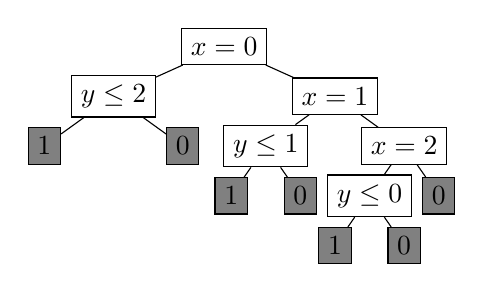
\begin{tikzpicture}
      [every tree node/.style={draw}, level distance=18pt,
      level 1/.style={sibling distance=80pt},
      level 2/.style={sibling distance=50pt},
      level 3/.style={sibling distance=25pt}]
      \node[draw] {$x = 0$}
        child {node[draw] {$y \leq 2$}
          child {node[fill=gray,draw] {$1$}}
          child {node[fill=gray,draw] {$0$}}
        }
        child {node[draw] {$x = 1$}
          child {node[draw] {$y \leq 1$}
            child {node[fill=gray,draw] {$1$}}
            child {node[fill=gray,draw] {$0$}}
          }
          child {node[draw] {$x = 2$}
            child {node[draw] {$y \leq 0$}
              child {node[fill=gray,draw] {$1$}}
              child {node[fill=gray,draw] {$0$}}
            }
            child {node[fill=gray,draw] {$0$}}
          }
        }
        ;
    \end{tikzpicture}
    \caption{Decision tree for predicates of size $3$}
    \label{fig:dt:large}
  \end{subfigure}
  \begin{subfigure}{0.5\textwidth}
    \centering
    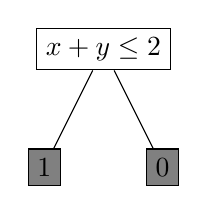
\begin{tikzpicture}
      \node[draw] {$x + y \leq 2$}
        child {node [fill=gray,draw] {$1$}}
        child {node [fill=gray,draw] {$0$}}
      ;
    \end{tikzpicture}
    \caption{Decision tree for predicates of size $4$}
    \label{fig:dt:small}
  \end{subfigure}
\end{figure}

\paragraph{Decision tree repair}
In Algorithm~\ref{algo:xxx}, we discard the terms and predicates that
are equivalent to already generated terms and predicates on the selected
points $\Points$ in lines~\ref{line:main:xxx},~\ref{line:main:yyy},
and~\ref{line:main:zzz}.
However, these discarded terms and predicates, may lead to better
solutions than the already generated ones.

\begin{example}
  Consider a run of the algorithm on the specification for the running
  example, where the set $\Points$ contains the points $\{ x \mapsto 1,
  y \mapsto 0 \}$ and $\{ x \mapsto -1, y \mapsto 0 \}$.
  Suppose the algorithm first generates the terms $0$ and $1$.
  These terms are each correct on one of the points and are added to
  $\Terms$.
  Next, the algorithm generates the terms $x$ and $y$.
  However, these are not added to $\Terms$ as $x$ (resp. $y$) is correct
  on exactly the same set of points as $1$ (resp. $0$).

  Suppose the algorithm also generates the predicate $x \leq y$ and
  learns the decision tree corresponding to the expression $\Expr \equiv
  \mathtt{if}~x \leq y~\mathtt{then}~0~\mathtt{else}~1$.
  Now, verifying this expression produces a counter-example point, say
  $\{ x \mapsto 1, y \mapsto 2 \}$.
  While the term $0$, and correspondingly, the expression $\Expr$ is
  incorrect on this point, the term $y$ which was discarded as an
  equivalent term to $0$, is correct.
\end{example}

Hence, for a practical implementation of the algorithm we do not discard
these terms and predicates, but store them separately in a map $\Equiv :
\Terms \to \Powerset{\Theory[\FormalParameters]}$ that maps the terms in
$\Terms$ to an additional set of equivalent terms.
At lines~\ref{line:main:xxx},~\ref{line:main:yyy},
and~\ref{line:main:zzz}, if the check for distinctness fails, we
instead add the term $\Term$ to the $\Equiv$ map.
Now, when the decision tree learning algorithm returns an expression
that fails to verify and returns a counter-example, we attempt to
replace terms and predicates in the decision tree with equivalent ones
from the $\Equiv$ map to make the decision tree behave correctly on the
counter-example.

\begin{example}
  Revisiting Example~\ref{ex:dt_repair}, instead of discarding the terms
  $x$ and $y$, we store them into the $\Equiv$ array, i.e., we set
  $\Equiv(0) = \{ y \}$ and $\Equiv(1) = \{ x \}$.
  Now, when the verification of the expression fails, with the
  counter-example point $\{ x \mapsto 1, y \mapsto 2 \}$, we check the
  term that is returned for the counter-example point--here, $0$.
  Now, we whether any term in $\Equiv(0)$ is correct on the
  counter-example point--here, the term $y$.
  If so, we replace the original term with the equivalent term that is
  additionally correct on the counter-example point and proceed with
  verification.
  Replacing $0$ with $y$ in the expression gives us $\mathtt{if}~x \leq
  y~\mathtt{then}~y~\mathtt{else}~1$.
  Another round of verification and decision tree repair will lead to
  replacing the term $1$ with $x$, giving us the final correct solution.
\end{example}

\paragraph{Branch-wise verification}
In Algorithm~\ref{algo:main}, and in most synthesis techniques, an
incorrect candidate solution is used to generate $1$ counter-example
point.
However, in the case of conditional expressions and point-wise
specifications, each branch can be verified separately.
Verifying each branch involves rewriting the specification as in the
point-wise verification defined in Section~\ref{sec:defs} -- but with the
added formula enfor
This gives us two separate advantages:
\begin{compactitem}
\item We are able to generate multiple counter-examples from a single
  incorrect expression.
  This reduces the total number of iterations required, as well as the
  number of calls to the expensive decision tree learning algorithm.
\item It reduces the complexity of each call to the verifier in terms of
  the size of the SMT formula to be checked.
  As verification procedures generally scale exponentially with respect
  to the size of the SMT formula, multiple simpler verification calls
  are often faster than one more complex call.
\end{compactitem}
This optimization works very well along with the decision tree repair
described above as we can verify and repair each branch of the decision
tree separately.

\begin{example}
  Consider the verification of the expression $mathtt{if}~x \leq
  y~\mathtt{then}~0~\mathtt{else}~1$ for the running example.
  Instead of running the full expression through the verifier and
  obtaining one counter-example point, we instead verify the two
  branches separately.
  This involves checking the satisfiability of the formulae $x \leq y
  \wedge f(x, y) = 0 \wedge \neg \Spec$ and $\neg (x \leq y) \wedge f(x,
  y) = 1 \wedge \neg \Spec$.
  This gives us two separate counter-example points as both branches are
  incorrect.
\end{example}

% \paragraph{Other optimizations}
% Bunching\dots
% Anything else?

\section{Evaluation}
\label{sec:evaluation}
% \begin{table}[!t]
\centering
\fontsize{8}{10}\selectfont
\begin{tabular*}{\linewidth}{@{\extracolsep{\fill}}lllcccccc}\\\hlx{hv}
\multirow{2}{*}{Benchmark} & Solution & Solution & DT & Max Term & Max Pred & Num \\
& Size & Time (s) & Size &  Size & Size & Points\\\hlx{hv}

icfp\_103\_10 & 33 & 8.9 & 7 & 4 & 6 & 9\\
icfp\_104\_10 & 17 & 0.8 & 5 & 3 & 5 & 6\\
icfp\_105\_1000 & 15 & 24.1 & 5 & 3 & 5 & 4\\
icfp\_105\_100 & 16 & 2.8 & 5 & 3 & 5 & 7\\
icfp\_113\_1000 & 11 & 35.5 & 3 & 4 & 4 & 2\\
icfp\_114\_100 & 20 & 154.6 & 5 & 5 & 5 & 3\\
icfp\_118\_100 & 31 & 13.8 & 7 & 4 & 5 & 4\\
icfp\_118\_10 & 32 & 3.4 & 7 & 4 & 5 & 6\\
icfp\_125\_10 & 57 & 9.6 & 13 & 4 & 6 & 10\\
icfp\_134\_1000 & 33 & 932.3 & 7 & 5 & 6 & 12\\
icfp\_135\_100 & 13 & 34.6 & 3 & 5 & 4 & 2\\
icfp\_139\_10 & 10 & 1.2 & 3 & 4 & 4 & 2\\
icfp\_143\_1000 & 16 & 903.8 & 3 & 5 & 5 & 3\\
icfp\_144\_1000 & 24 & 876.1 & 5 & 5 & 6 & 3\\
icfp\_144\_100 & 36 & 477.8 & 7 & 5 & 6 & 16\\
icfp\_147\_1000 & 12 & 661.8 & 3 & 5 & 4 & 2\\
icfp\_150\_10 & 51 & 1.7 & 11 & 4 & 5 & 6\\
icfp\_21\_1000 & 21 & 302.4 & 5 & 4 & 5 & 5\\
icfp\_25\_1000 & 22 & 92.8 & 5 & 4 & 6 & 8\\
icfp\_28\_10 & 2 & 0.03 & 0 & 2 & 0 & 1\\
icfp\_30\_10 & 14 & 10.2 & 3 & 5 & 4 & 4\\
icfp\_32\_10 & 14 & 8.5 & 3 & 5 & 4 & 2\\
icfp\_38\_10 & 21 & 4.9 & 5 & 4 & 5 & 5\\
icfp\_39\_100 & 12 & 10.6 & 3 & 4 & 5 & 2\\
icfp\_45\_1000 & 9 & 16.9 & 3 & 3 & 4 & 2\\
icfp\_45\_10 & 9 & 0.12 & 3 & 3 & 4 & 2\\
icfp\_5\_1000 & 19 & 44.1 & 5 & 3 & 5 & 4\\
icfp\_51\_10 & 11 & 1.7 & 3 & 4 & 4 & 2\\
icfp\_54\_1000 & 11 & 25.1 & 3 & 4 & 4 & 2\\
icfp\_64\_10 & 21 & 26.7 & 5 & 5 & 5 & 5\\
icfp\_68\_1000 & 26 & 26.9 & 7 & 3 & 5 & 5\\
icfp\_69\_10 & 11 & 1.1 & 3 & 3 & 5 & 5\\
icfp\_7\_1000 & 17 & 61.8 & 5 & 3 & 6 & 9\\
icfp\_7\_10 & 16 & 0.76 & 5 & 3 & 5 & 6\\
icfp\_72\_10 & 13 & 14.4 & 3 & 5 & 4 & 2\\
icfp\_73\_10 & 18 & 0.51 & 5 & 3 & 5 & 3\\
icfp\_81\_1000 & 21 & 382.4 & 5 & 4 & 5 & 7\\
icfp\_82\_100 & 13 & 8.9 & 3 & 3 & 6 & 8\\
icfp\_82\_10 & 13 & 3.5 & 3 & 3 & 6 & 7\\
icfp\_87\_10 & 19 & 5.2 & 5 & 4 & 5 & 5\\
icfp\_93\_1000 & 22 & 127.5 & 5 & 4 & 5 & 9\\
icfp\_94\_1000 & 17 & 29.5 & 5 & 3 & 5 & 4\\
icfp\_94\_100 & 17 & 2.4 & 5 & 3 & 5 & 4\\
icfp\_95\_100 & 220 & 182.5 & 55 & 4 & 7 & 55\\
icfp\_96\_1000 & 49 & 1289.8 & 11 & 5 & 6 & 22\\
icfp\_96\_10 & 57 & 9.5 & 13 & 4 & 6 & 9\\
icfp\_99\_100 & 18 & 201.2 & 5 & 5 & 5 & 4\\
icfp\_14\_1000 & -- & TO & -- & -- & -- & --\\
icfp\_56\_1000 & -- & TO & -- & -- & -- & --\\
icfp\_9\_1000 & -- & TO & -- & -- & -- & --\\\hlx{hv}
\end{tabular*}

\end{table}

\begin{table}
\centering
\fontsize{9}{11}\selectfont
\begin{tabular*}{\linewidth}{@{\extracolsep{\fill}}lllllllc}\\\hlx{hv}
\multicolumn{1}{c}{\multirow{2}{*}{Benchmark}} & \multicolumn{1}{c}{Size} & \multicolumn{1}{c}{Time} & \multicolumn{1}{c}{DT Size} & \multicolumn{1}{c}{Size} & \multicolumn{1}{c}{Time} & \multicolumn{1}{c}{DT Size} & Min\\
& \multicolumn{1}{c}{of first} & \multicolumn{1}{c}{to first} & \multicolumn{1}{c}{for first} & \multicolumn{1}{c}{of min} & \multicolumn{1}{c}{to min} & \multicolumn{1}{c}{for min} & first?\\\hlx{hv}
icfp\_103\_10 & 33 & 12.1 & 7 & 26 & 427.4 & 5 & $\times$\\
icfp\_104\_10 & 17 & 1.1 & 5 & 17 & 30.9 & 5 & $\times$\\
icfp\_105\_1000 & 15 & 35.9 & 5 & 11 & 134.9 & 3 & $\times$\\
icfp\_105\_100 & 16 & 3.1 & 5 & 12 & 9.1 & 3 & $\times$\\
icfp\_113\_1000 & 11 & 53.6 & 3 & 11 & 53.6 & 3 & $\checkmark$\\\hlx{h}
icfp\_114\_100 & 20 & 241.6 & 5 & 21 & 793.1 & 5 & $\times$\\
icfp\_118\_100 & 31 & 18.1 & 7 & 16 & 135.8 & 3 & $\times$\\
icfp\_118\_10 & 32 & 4.1 & 7 & 15 & 9.1 & 3 & $\times$\\
icfp\_125\_10 & 57 & 8.8 & 13 & 14 & 437.3 & 3 & $\times$\\
icfp\_134\_1000 & 33 & 1441.1 & 7 & 27 & 2437.4 & 5 & $\times$\\\hlx{h}
icfp\_135\_100 & 13 & 54.0 & 3 & 13 & 54.0 & 3 & $\checkmark$\\
icfp\_139\_10 & 10 & 1.3 & 3 & 10 & 1.3 & 3 & $\checkmark$\\
icfp\_14\_1000 & -- & TO & -- & -- & TO & -- & -- \\
icfp\_143\_1000 & 16 & 1412.5 & 3 & 16 & 1412.5 & 3 & $\checkmark$\\
icfp\_144\_1000 & 24 & 1376.8 & 5 & 24 & 1376.8 & 5 & $\checkmark$\\\hlx{h}
icfp\_144\_100 & 36 & 763.5 & 7 & 26 & 2810.3 & 5 & $\times$\\
icfp\_147\_1000 & 12 & 1114.3 & 3 & 12 & 1114.3 & 3 & $\checkmark$\\
icfp\_150\_10 & 51 & 1.7 & 11 & 24 & 9.3 & 5 & $\times$\\
icfp\_21\_1000 & 21 & 512.6 & 5 & 20 & 1099.5 & 5 & $\times$\\
icfp\_25\_1000 & 22 & 151.6 & 5 & 15 & 1571.4 & 3 & $\times$\\\hlx{h}
icfp\_28\_10 & 2 & 0.04 & 0 & 2 & 0.04 & 0 & $\checkmark$\\
icfp\_30\_10 & 14 & 14.4 & 3 & 14 & 14.4 & 3 & $\checkmark$\\
icfp\_32\_10 & 14 & 9.1 & 3 & 14 & 9.1 & 3 & $\checkmark$\\
icfp\_38\_10 & 21 & 5.9 & 5 & 14 & 54.1 & 3 & $\times$\\
icfp\_39\_100 & 12 & 15.8 & 3 & 12 & 15.8 & 3 & $\checkmark$\\\hlx{h}
\end{tabular*}
\vspace*{1mm}
\caption{Results on the ICFP benchmark suite. All times are in seconds.}
\label{table:anytime_results_1}
\end{table}

\begin{table}[!t]
\centering
\fontsize{9}{11}\selectfont
\begin{tabular*}{\linewidth}{@{\extracolsep{\fill}}cllllll}\\\hlx{hv}
\multirow{2}{*}{\# Args} & \multicolumn{3}{c}{D\&Q Enumeration} & \multicolumn{3}{c}{CVC4}\\\hlx{vc{2-4,5-7}v}
& Size & Time (s) & \# Comp. & Size & Time (s) & \# Comp\\\hlx{h}
2 & 6 & $< 0.1$ & 1 & 6 & $< 0.1$ & 1\\
3 & 16 & 0.16 & 3 & 25 & $< 0.1$ & 4\\
4 & 36 & 0.77 & 7 & 55 & $< 0.1$ & 9\\
5 & 76 & 6.2 & 15 & 96 & $< 0.1$ & 16\\
6 & 156 & 63.2 & 31 & 148 & $< 0.1$ & 25\\
7 & 316 & 546 & 63 & 211 & $< 0.1$ & 36\\
8 & -- & TO & -- & 285 & $< 0.1$ & 49\\
9 & -- & TO & -- & 370 & 0.1 & 64\\
10 & -- & TO & -- & 466 & 0.15 & 81\\\hlx{h}
\end{tabular*}
\caption{Results on the parameterized ``max'' benchmarks.}
\label{table:max_results}
\end{table}


We built a prototype \sygus solver based on the ideas presented in
this paper. The algorithms for enumeration were implemented in
about 3000 lines of Python code, while the algorithms for decision
tree learning were implemented in about 3000 lines of
C$\raisebox{1pt}{+\!+}$ code. All experiments were executed on a
32-core machine with four Intel Xeon E7-4820 processors running at 2.0
GHz, and 128 GB of memory, with a one hour time limit.

This section first sets up the questions that we would like for our
experimental evaluation to answer, We then briefly describe
the benchmarks used and comment on the state-of-the-art in solving
these benchmarks, to provide some context to the reader.
We then conclude this section with a discussion about our
experimental observations.

\subsection{Goals, Benchmarks and the State-of-the-art}
\paragraph{Goals}
We seek to empirically evaluate how our synthesis algorithm compares
to other state-of-the-art synthesis techniques along the following
dimensions:
\begin{inparaenum}[(a)]
\item
\emph{Performance}: How quickly can the algorithms arrive at a correct
solution?
\item
\emph{Quality}: How \emph{good} are the solutions produced by the
algorithms? We use compactness of solutions, in terms of syntactic
size, as a metric for the quality of solutions.
\item
\emph{Effect of continued execution}: How significant is the
improvement in the quality of the solutions generated if the
algorithm is given an additional (but fixed) time budget.
\end{inparaenum}

\paragraph{Benchmarks}
To compare and contrast the \dcsolve algorithm with contemporary
techniques along each of these dimensions, we considered two classes
of \sygus benchmarks. We did not consider the other classes in the
general-track \sygus benchmarks because:
\begin{inparaenum}[(a)]
\item the solutions were not conditional expressions, as is the case
with the bit-vector benchmarks, or
\item the benchmarks were not plainly separable, or
\item the benchmarks were very similar to the ones that we have
considered.
\end{inparaenum}
The first class that we considered consists of the ICFP
benchmarks. These are bit-twiddling problems, with very specific
restrictions on the bitwise operations that are allowed. The behavior
of the function to be synthesized is specified only using concrete
input-output examples. To the best of our knowledge, no existing
\sygus solver has been able to solve these benchmarks. The results of
running our solver on these benchmarks is summarized in
Table~\ref{table:anytime_results}. The first column of
Table~\ref{table:anytime_results} gives the name of the benchmark, the
second and third columns give the size of the earliest solution
discovered by the algorithm, the time taken to discover the solution,
and the size of the decision tree associated with the solution,
respectively. The next three columns provide the same details, but for
the \emph{minimal} sized solution discovered by the
algorithm. Finally, the last column indicates whether the solution
that was discovered earliest was also the solution with the minimal
size. The second class of benchmarks that we considered compute the
maximum of $n$ integers, where $n$ is a
parameter. Table~\ref{table:max_results} demonstrates how our
algorithm stacks up against the state-of-the-art CVC4 solver. The
columns indicate the sizes of solutions generated, the time to arrive
at the solution, as well as the number of comparisons in the solution
obtained by each of the solvers, for different values of the parameter
$n$, indicated in the first column.

\paragraph{The State-of-the-art}
One can broadly categorize the existing \sygus solvers into two
categories:\begin{inparaenum}[(a)]
\item
\emph{Black-box solvers}, which do not leverage the correctness
specification to guide the search for solutions. Some examples are
\esolver and the stochastic solver~\cite{udupa-sygus}, as well as the
\dcsolve algorithm.
\emph{White-box solvers}, which actively leverage the correctness
specification to generate terms and predicates for solutions. Examples
for white-box solvers include the solvers based on the \textsc{stun}
algorithms~\cite{ACR15}, and the CVC4 solver~\cite{reynolds-15}.
\end{inparaenum}
Empirically, black-box algorithms are able to generalize well from
underconstrained correctness specification, whereas it is not clear
how white-box solvers can generalize from such specifications, given
their heavy reliance on the specifications being complete.
We note that \esolver, which employs an optimized
version of the na\"ive enumerative algorithm discussed earlier won the
2014 \sygus competition and came in second in the 2015 \sygus
competition, losing to the CVC4 solver, which came in first.

\subsection{Discussion}
Having set the context with respect to the benchmarks and contemporary
solvers, we now proceed to a discussion on how the
\dcsolve algorithm compares to contemporary solvers along the three
dimensions described earlier.

\paragraph{Performance}
As Table~\ref{table:anytime_results} demonstrates, our algorithm was
able to produce a solution for 47 out of the 50 ICFP benchmarks,
within an hour. We emphasize that we know of no other solver that has
been able to provide satisfactory solutions to these
benchmarks. Further, as Figure~\ref{figure:random_exponential_graph}
indicates, it would be impossible to explore expressions of the size
indicated in Table~\ref{table:anytime_results} --- which are often
larger than 20 --- using a na\"ive enumeration strategy, such as the
one used by \esolver.  The solutions produced by our divide and
conquer algorithm are quite compact, and most of them are computed in
less than ten minutes, with only five benchmarks taking longer.

Table~\ref{table:max_results} indicates that our algorithm is competitive
with the state-of-the-art CVC4 solver on the parameterized ``max of
$n$ numbers'' benchmarks, for smaller values of $n$. For larger
values of $n$, our algorithm is not as performant. Our investigations
indicated that in the performance drops are largely due to the large
number of concrete counterexample points that the algorithm maintains,
which in turn leads to the decision tree learning algorithms taking
longer.

To summarize, the \dcsolve algorithm demonstrates vastly better
performance than other black-box solvers. Its performance is
competitive with white-box solvers, while also being able to
generalize well from input-output examples as we will now discuss.

\paragraph{Quality of Solutions}
In the case of the ICFP benchmarks, Table~\ref{table:anytime_results}
indicates that most of the solutions that our algorithm generates are
rather compact, and are of a size that are comprehensible to a
human. We do not know if solutions smaller than these exist. The CVC4
solver has been able to synthesize solutions for some of the ICFP
benchmarks, but only when syntactic restrictions are lifted. However,
upon closer inspection, we discovered that the solutions were just a
large case-split corresponding to the input-output examples that form
the constraints for the problem. Although technically correct, the
solutions are extremely large, perform no generalization and are
unlikely to be the intended or desired solutions. We emphasize
that no solution generated by our algorithm is a similar large
conditional expression that matches inputs to outputs. The solutions
that we report are all compact expressions that perform some
computation on the input, to return an output.

In the case of the ``max'' benchmarks, we again see from
Table~\ref{table:max_results} that our algorithm performs well for
small parameter values, often beating the solutions obtained from the
CVC4 solver in terms of size and number of comparisons. At larger
parameter values, the solutions are still reasonably compact and not
excessively large. The reason for the somewhat larger solutions for
larger parameter values is that the decision tree learning algorithm
is not optimal, \ie, it does not guarantee the most compact decision
tree. Instead a greedy heuristic is used, which rapidly yields
suboptimal solutions as the number of samples (counterexample points)
increases, as with the ``max'' benchmarks for larger
parameter values. We intend to explore how we can adapt other
heuristics~\cite{Madhu}, into the setting of our problem, in future
work.

\paragraph{Effect of Continued Execution}
We observe from the last column in Table~\ref{table:anytime_results}
that for about half the ICFP benchmarks, we were able to obtain a more
compact solution by continuing to execute our algorithm even after the
first solution was discovered. Also, the difference in the first and
smallest solutions is sometimes very significant, for example, in the
case of the ``icfp\_95\_100'' benchmark, we see the size of the
solutions go down by almost an order of magnitude, from 220 to 24. An
interesting phenomenon that we observed was that our algorithm would
sometimes find \emph{larger} solutions when allowed to run
longer. However, we observed that the size of the decision trees
almost always reduced with time. It turns out that although the
decision trees learned were smaller, running the algorithm longer also
meant that larger terms and predicates were enumerated, thus leading
to the overall expression sizes of the solutions to sometimes increase
with time.

Our experimental evaluation thus allows us to draw the following
conclusions:
\begin{inparaenum}[(a)]
\item
The \dcsolve algorithm is able to quickly learn compact solutions for
a large fraction of the ICFP benchmarks, and generalizes well from
input-output examples.
\item
The anytime nature of the \dcsolve algorithm is often useful in
reducing the size of the computed solution by allowing additional
execution time.
\item
The \dcsolve algorithm works competently on problems from other
classes of benchmarks that admit conditional expressions as solutions,
such as the parameterized ``max'' benchmarks.
\end{inparaenum}

\section{Concluding Remarks}
\label{sec:conclusion}

\subsection{Related Work}
\begin{itemize}
\item
Connection to ``classical synthesis'' techniques like sketch, cegis in general
\item
Connection and contrast with Madhu's decision tree work, ICE-DT
\item
Jha's loop free synthesis (ICSE '10, PLDI '11)
\item
Gulwani's flash* stuff
\item
Peter Michael Osera's dissertation (synthesis using type theory stuff)
\item
Superoptimization (Denali, Massalin), Stochastic superoptimization.
\item
Ruzika, Viktor's work
\item
Sumit's recursive program crap
\end{itemize}
\subsection{Conclusion}

\bibliographystyle{plainnat}
\setlength{\bibsep}{1pt}
\begin{small}
\bibliography{main}
\end{small}

\arsays{Madhu's work assumes that the predicate domain can distinguish
any two points?}

\end{document}
